\newcommand{\defNode}[1]{%
  \expandafter\def\csname nd#1\endcsname{\emph{#1}\xspace}}
\newcommand{\defNodes}[1]{\forcsvlist{\defNode}{#1}}

\chapter{Incremental Deployment}
In this chapter, we present the \tincdep we introduced for further extension or optimisation of \dpy. We first present why we introduce \tincdep. After that, each section of this chapter contains one main aspect of \tincdep, including the expected behaviour of \tincdep, the semantics changes due to \tincdep and how \tincdep works, except for the last two sections - the second last section presents an example of \tincdep, and the last section presents how we implement \tincdep in \dpy (including what issues we encountered and how we solved them).

We expect, as said in the Background chapter, future researchers would need to design workflows reading data from continuous infinite, on the basis of units, data sources. In this situation, the execution time of the workflow will also be infinite unless manually shut down. Therefore, it is infeasible to use past performance data from an ``infinite workflow'' to guide the deployment of future runs of the same workflow. A more dynamic on-the-fly way of deploying PEs to nodes is needed to support possible optimisations. This is one of the reasons we introduce \tincdep.

The other reason is that we expect to support a more natural way to design workflows to accomplish tasks such as the \tsieve we discussed in the Use Case chapter. Details of why we need \tincdep to support it will be discussed in \tDynExp chapter.

There is also another reason: we want to minimize the initialization cost for the execution of workflows and spawning, connecting and deploying nodes cost lots of resources, especially time. We expect doing all of spawning and deployment on-the-fly can save time in some cases.

\section{Deployment Behaviour}
As \tincdep is the new extension we introduced, we shall first describe the expected behaviour of it as well as a brief comparison against the old system.

In the current \dpy system, when \dpy wants to deploy \tPEInst to nodes, it will first analyse the workflow to extract the topology and then map \tPEInst{}s to nodes and leave them executing without any more management. The number of nodes used in execution should be assigned prior to execution and is not subject to change during execution.

We want to introduce more dynamic behaviours, so our expected behaviour should be like this:
\begin{enumerate}
	\item The user doesn't need to know the actual number of nodes needed to execute a workflow (however, the user \emph{can} know that).
	\item \Dpy will deploy and run only the source \tPEInst{}s in the beginning, rather than all \tPEInst{}s at once.
	\item Other \tPEInst{}s will be deployed during running and each \tPEInst should be deployed exactly once so data transmission won't go wrong because of this late-deploy behaviour.
	\item When a unit of data is going to be sent through an output connection, it will go to the correct destination.
	\item If the output connections of more than one \tPEInst{}s are connected to the same input connection of another \tPEInst, the data sent through these output connections will go to (the same input connection of) the same \tPEInst.
	\item A \tPEInst should shutdown when there is no more data to produce.
	\item If a \tPEInst never receives any data from any input connections, this \tPEInst doesn't need to be deployed.
\end{enumerate}

To satisfy all these needs, especially the 2nd and 5th points, we need a mechanism to synchronize the knowledge of \tPEInst{}s so no duplicated deployment or lost of data will happen. Because of the nature of distributed computing, we couldn't, at least during the time, find a low-cost way (\ie without many signalling rounds) to guarantee these requirements in a fully de-centralized manner. Therefore, we introduced a coordinator to handle the deployment. We will show, in the Coordinator section below, that our communication strategy is the minimal possible.

To put all these together, the deployment behaviour now is:
\begin{enumerate*}
	\item The coordinator will be launched first in the beginning
	\item The coordinator analyses the workflow and deploys the source \tPEInst{}s (\ie \tPEInst{}s without any explicit input connections).
	\item the coordinator deploys the successor \tPEInst to a node when a \tPEInst needs to send data through an output connection which is connected to a input connection of the successor.
\end{enumerate*}

\section{Revised Semantics for Sending Data}
We briefly mentioned when sending data through an output connection, the coordinator is responsible for deploying the successor \tPEInst{}(s). Here we present how the semantics for sending data has changed and how this is reflected in out implementation of sending data.

In the old \dpy system, because all \tPEInst{}s are deployed in the beginning, all nodes are completely aware with which input connection of which node is an output connection connected. As a result, when an output is produced, the node knows naturally where it will go to. However, because \tPEInst{}s are deployed dynamically when we introduce \tincdep, all nodes lose this knowledge so this semantics is subject to change.

In \tincdep, when a \tPEInst produces a unit of data and sends it through an output connection, this action triggers a lookup to find the correct targets (both input connections and nodes). If the targets haven't been deployed yet, the send action will hang up to wait for the completion of the deployment (which is performed by the coordinator) of the targets and then the send action proceeds.

In our implementation, when a \tPEInst produces a unit of data, the node (which runs the \tPEInst) will communicate with the coordinator to request the destination(s) of the output connection. Then it waits for the reply from the coordinator to tell it where that data should be sent to. When it receives the reply, it caches the information (reply) and when next time it is going to send data through the same output connection, it will use the cached information instead of communicating with the coordinator a second time. 
The deployment strategy and process is hidden to the execution nodes, so their main job is still executing the \tPEInst.

It is clear that in this strategy we only add an inspection to the procedure for sending data: to acquire the destination from the coordinator the first time an output connection is used. The rest part of the existing procedure remains unchanged.

\section{Target Selection of Deployment}
What happens during the time the execution node waits for the reply from the coordinator? The coordinator finds the successor \tPEInst{}s which have input connections connected to that output connection, and deploys the \tPEInst{}s to some nodes.

The step to find the successor \tPEInst{}s is fairly simple: the input and output connection pairs are seen as edges in a graph and the coordinator did a topological sort in the beginning so it can barely lookup the result.

When the coordinator knows the successor \tPEInst{}s, it will need to deploy them correspondingly to some nodes. In our system, we perform a plain lookup in the table which contains the status (busy or free) of nodes, and use the first enough free nodes. We are aware that there is a potential optimisation for selecting the nodes to deploy the \tPEInst{}s, such as considering the network speed between the nodes, or considering the computational capability of nodes. However, because of the time limit, it is not possible to accomplish it in our MSc project.

During the lookup, if there is no enough nodes available (free), the coordinator will spawn more nodes and try again. We can use different strategies to decide the number of nodes to be spawned, but we only use a constant for now.

\section{Coordinator}
The above two sections only talked about the general role of the coordinator. In this section, we present the actual behaviour of the coordinator during deployment.

The coordinator first performs a topological sorting to the workflow graph in the beginning, and stores which output connection (and the \tPEInst) is connected with which input connection in a quick lookup table (hash table). It then deploys the source nodes which have no input connections (\ie zero in-degree). The coordinator stores a record (array) which keeps the status of every execution nodes, to track whether they are busy (has a \tPEInst deployed deployed at the moment) or free (has no \tPEInst deployed at the moment), and also the \tPEInst each busy node is running.
Then, the coordinator waits for signals (\ie communications) from the execution nodes after sources are deployed.

During waiting, when the coordinator receives a signal which requires the successors of an output connection, it lookups what input connections and \tPEInst{}s are connected with this output connection, and then checks each of the \tPEInst{}s in the record to see if it is already deployed. For each of those undeployed \tPEInst{}s, the coordinator will deploy it to a node and record this deployment. After all these \tPEInst{}s are deployed, the coordinator replies the requester with the input connections and the nodes where these \tPEInst{}s are deployed.

It is apparent that there is no need for a node to request for the successors of the same output connection more than once because the deployment won't be changed, so each execution node will cache the reply (or any modifications to the reply) locally. It is also apparent that there is no need for the coordinator to send an ``ack'' back to the requester when receiving the request or for the requester to send an ``ack'' back to the coordinator when receiving the reply from the coordinator, because there is no subsequent actions after each of these signals as long as we can guarantee each message will eventually arrive (which is true under MPI).

When deploying the \tPEInst, the coordinator sends the information necessary for a node to construct the \tPEInst. In our implementation, we assign an unique ID for each \tPEInst in the workflow and all nodes possess the knowledge of the workflow. Therefore, the coordinator simply sends the ID of the target \tPEInst to the node and the node directly looks up the \tPEInst in the workflow and execute it. We can think of an alternative method which may be more flexible: send instructions/information necessary to construct the \tPEInst from \tPETmpl to the target node (and also adjust the workflow not to directly use \tPEInst{}s but to use construction information of every \tPEInst{}), so the coordinator can modify these instructions/information if needed. However, because we are constrained by time, we only implemented a backward-compatible method.

\section{Shutdown Process}
The execution should be able to begin, and should also be able to shutdown properly. In this chapter, we describe how the shutdown process works.

\newcommand{\dEOS}{end-of-stream\xspace}

In the existing \dpy system, the shutdown process is done by performing forward shutdown propagation. It consists of the following steps:
\begin{enumerate}
	\item When a \tPEInst has no more data to produce (e.g. because it is the source process and it has produced all data it is designed to produce), it will send an ``\dEOS'' marker through all output connections. Then it shuts itself down.
	\item These \dEOS markers will then be received by the successor \tPEInst{}s and they will decide whether all inputs have received enough numbers of the \dEOS marker.
	\item If all input connections have received enough \dEOS markers, the \tPEInst will propagate the \dEOS markers to all output connections, and shuts itself down (same as step 1).
\end{enumerate}

We used an attributive, ``enough'', for correctness in case an input connection has more than one output connections connected. This can be done by using several counters each for one input connection to count for the number of \dEOS received. Furthermore, because the shutdown process works as a whole for the \tPEInst, we don't need a separate counter for each input connections, but only need a total counter for all input connections. More details of the counter will be described in the Lazy Deployment section below.

By using this method, all nodes will be guaranteed to shut down correctly when there is no more job to do and therefore no more data to produce. We keep this behaviour in our extension (with one difference which will be described in the Lazy Deployment section) so the coordinator doesn't need to propagate shutdown signals.

But we'd like the coordinator to be aware of the status of all nodes so it can re-deploy other \tPEInst{}s to a node which has previously shut down so the resources will be better used. Therefore, we add an additional signal to tell the coordinator that a node is shutting down now. When the coordinator receives this signal, it then marks the signal source as free so the coordinator can re-deploy other \tPEInst{}s to it.

\section{Backward Shutdown Propagation}
TO BE CONSTRUCTED

\section{Lazy Deployment}
Lazy deployment is not a specially designed feature, but a natural feature emerged during the implementation of \tincdep.

As the process of deployment shows, the existing \dpy system will deploy all \tPEInst{}s to all nodes. However, because of the variety and uncertainty of incoming data, sometimes some \tPEInst may never receive any units of data. Therefore, it is not needed to deploy them to nodes. If this is a whole branch of the workflow (because of, \eg, this branch is for debugging), by not deploying these \tPEInst{}s, many nodes can be saved.

With the existence of lazy deployment, \tPEInst{}s will be deployed only if they are needed. This behaviour is the same behaviour of the deployment strategy of \tincdep - that's why we say lazy deployment is naturally emerged.

Because of the existence of lazy deployment, it seems the behaviour of shutdown propagation should be changed slightly. The most natural way for propagating the shutdown signal is: each \tPEInst still propagates the \dEOS signal to all output connections, but only those output connections which has successors deployed will actually send out the \dEOS signal, in order not to trigger a deployment. However, because we need a counter to count for the number of \dEOS{}s from all input connections in order to guarantee the propagation works correctly in the presence of multi-to-one connections, we need another mechanism to guarantee the counter works correctly in lazy deployment. We argue that it is impossible, in a distributed asynchronous system, to guarantee the counter works correctly without doing round communications with the coordinator (\eg, probing to and answering from the coordinator whether it is able to shut down). A simple example is enough to demonstrate (see Figure \ref{fig:incdep_lazydep_0}):

\defNodes{O,A,B,S}

\ndO (for \emph{Origin}) produces some number. If the number is odd, it is sent through \lstinline|output1| which is connected to \lstinline|input| of \ndA; if the number is even, it will be sent through \lstinline|output2| which is connected to \lstinline|input| of \ndB. \ndA and \ndB perform some calculation to the data they receive and send them to \ndS (both through their \lstinline|output| connection to the \lstinline|input| connection of \ndS). \ndB delays for some time (e.g. 2 seconds) before it can output data. \ndA finishes producing data immediately after producing the first unit of data. \ndS (for \emph{Sink}) does nothing but counting the number of units of data it receives.

\begin{figure}[h]
\centering
    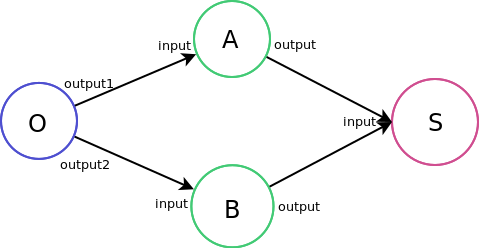
\includegraphics[width=0.8\textwidth]{figures/incdep_lazydep_0}
	\caption{Example figure for illustration in lazy deployment}
	\label{fig:incdep_lazydep_0}
\end{figure}

Apparently \ndS should wait until \ndB propagates the \dEOS marker if \ndB is deployed; \ndS shouldn't wait for the \dEOS marker if \ndB is not deployed. The basic way of tackling this requirement is \ndS checks (\ie probe) whether it is safe to shut down when it receives an \dEOS marker and wait for the reply (\ie answer) to tell it whether it is true or not, which requires a round communication each time \ndS receives a \dEOS (using a counter doesn't help in this scenario because there is no guarantee when the signal to increase the counter will arrive).

There are two options if we don't do probing and answering:
\begin{enumerate}
	\item Increase the to-be-waited number of nodes (by sending signals from the coordinator) for the input connections each time when a new node requires to output through a connection connected to that input connection.
	\item Set the number of nodes to-be-waited to the total possible number of nodes in the beginning.
\end{enumerate}

If we choose method 1, if \ndB delays for a long time and then tries to send data through output connection to \ndS, \ndA will have already finished. In this scenario, the to-be-waited number in \ndS before \ndB requires to send data is \emph{1}, so when \ndA broadcasts \dEOS, \ndS finds the number of total nodes finished has reached \emph{1} so it shuts itself down. A naive, but faulty, patch for this will be set the to-be-waited number larger (e.g. add one) than the actual number, but this will fail when there are more than one nodes requiring to send data at the same time (and finishing sending data before the sink node has received the signals telling it to increase that to-be-waited number. The only way to solve the problem in this method is (with the counter add-by-one in the beginning) to make the coordinator tell the sink that there is another node who will send data to you and wait for \textit{ack} from the sink, which requires round communication between the coordinator and the sink each time for each input connection.

If we choose the second method, when a branch, \eg \ndB, is not (and will never be) deployed because of lazy deployment, the \ndS will never receive the \dEOS from \ndB so the counter will never reach the desired number so the shutdown propagation will fail. The only way to solve this dilemma is to make the coordinator aware when it is the time for \ndS to shut down and tell it to shut down. However, if we choose this approach, it requires more calculations in the coordinator side, which doesn't match our desire to keep the workload of coordinator minimal and will more easily make the coordinator a bottleneck, and there is no need to keep the shutdown propagation because the coordinator now takes control of everything.

What we choose is to also deploy those \tPEInst{}s which are not deployed due to lazy deployment during shutdown propagation. We argue that this method won't create lots of overheads because the coordinator can re-assign these \tPEInst{}s to nodes which has previously shut down. We are aware that there is an extension to this approach which may significantly reduce the number of nodes deployed during the propagation process: do not deploy \tPEInst{}s (and their successors) whose successors (in any depths) will never have input connections connected with the output connections from other parts of the graph. However, because of the time limit, we didn't introduce this to our implementation.

\section{Simple Example}
Here we present a simple solid example to demonstrate how \tincdep works.

Consider a graph doing some simple mathematical calculations like this (see Figure \ref{fig:incdep_example_0}):
  
\defNodes{A,B,C,D,E}

\begin{itemize}
	\item Two nodes \ndA and \ndB each produces some numbers.
	\item Node \ndC splits the number by their sign: the positive ones go to node \ndD; the negative ones go to node \ndE.
	\item Node \ndD sums all positive numbers together.
	\item Node \ndE counts the number of data it receives.
\end{itemize}

\begin{figure}[h]
	\caption{HERE IS A FIGURE TO ILLUSTRATE THE TOPOLOGY OF THE EXAMPLE}
	\label{fig:incdep_example_0}
\end{figure}

\section{Implementation}
(NEEDS REVISION)

The sections above all describe about the design of the logic, rather than the implementation. In this section, we describe the issues we encountered during implementation. We will first talk about our design of the extension to \dpy, and then present the issues we encountered in each relevant subsection.

Because \tPEInst{}s are unaware of which node its input or output connections are connected to, they can't be executed plainly. The existing \dpy mechanism uses wrappers on each \tPEInst to handle the input, output and shutdown issues. We keep this design and do some extra work to make the wrapper run correctly under our extension.

\Dpy supports a mechanism called ``grouping'' so we need also provide mechanisms to support it when implementing our extension in order to keep backward compatibility.

\subsection{Efficiency, Concurrency, and Synchronization}
Because all nodes are executed in parallel, the time when a signal or a unit of data will arrive is unpredictable. Therefore, we need to guarantee the correctness under all circumstances. 

For example, when a \tPEInst is going to send a unit of data, it is possible that the reply from the coordinator returns immediately or it is also possible that the reply returns only after a long delay. Usually, sending data is a lot less computational-intensive than processing data. Therefore, it is usually more efficient to keep processing more data and leave the waiting and sending in concurrent.

We use multi-threading to achieve concurrency in the wrapper of \tPEInst, and keep the design of each \tPEInst intact (they will usually be designed in a single-threaded manner); the coordinator is also change to multi-threaded for better performance.

We can expect many communication to and from the coordinator run in parallel. Therefore, we will handle each request in a separate thread. Because multiple requests may act on a same PE, we will add a lock to each PE and acquire it when it is going to be act on (and release it when finished) so different requests of this same PE will be sequentialized.

Because a wrapper reads data from some input connections, processes the data previously read in the \tPEInst it wraps and writes processed output to some output connections, we run ``read'' in one thread, and run ``process'' and ``write'' together in another thread. If the order of data doesn't matter, we will run both ``process'' and ``write'' in several threads (in a thread pool). Because we need also request the address of targets (successor nodes), we need to design a suitable place to handle the communication to the coordinator. We decide to send the request at where is needed, and listen in another dedicated thread. The synchronous will be done by using condition variables - wait for the condition variable to become true after sending the request, and set it to true when receiving the reply.

\subsection{Spawning}
One of the possibilities \tincdep gives \dpy is it allows to spawn more nodes when needed (\eg initial nodes are not enough). However, this behaviour also increases the complexity of the code.

Three aspects are affected by supporting spawning:
\begin{enumerate}
	\item Determine and spawn new nodes.
	\item Establish communication between existing and new nodes.
	\item Select the right channel to transmit data / message.
\end{enumerate}

\subsubsection{Determine and Spawn}
Determining when to spawn new nodes is fair easy: the coordinator simply checks if there are enough free nodes to be assigned the required \tPEInst{}s. If there aren't enough free nodes, it is very \textbf{likely} the coordinator needs to spawn more nodes. We emphasize the word \textbf{likely} because sometimes there is no need to spawn: for example, when the whole workflow is a line and the data is finite, the head node will finish so the coordinator can wait until its finishing and re-deploy next \tPEInst to it. However, this behaviour is not steady so we force the coordinator to spawn more nodes once a short-of-node happens.

We need to ensure all nodes are communicable, so, under MPI specification, all nodes need to collectively spawn the new nodes. This involves a message transmission from the coordinator to make worker nodes aware there is a node to spawn and trigger the spawning function call.

\subsubsection{Establish Communication}
We expect all nodes (at least, all worker nodes) to be able to communicate with each other. We choose to merge the new \emph{Intercommunicator} created by the spawning process into one larger \emph{Intracommunicator}. In this way, we can use repeat the same behaviour for spawning more nodes though the newly created \emph{Intracommunicator}.

To suit the existing grouping mechanism, which is introduced to increase throughout by (automatically) deploying \tPEDup{}s of the same \tPEInst and processing data in parallel, we use local leaders (called \textbf{representative}) for each group. The representative is responsible for synchronization between groups.

As a result, we use three sets of communicators: one for data transmission, one for communication between the coordinator and the worker nodes and one for communication inside each group. We use \lstinline|Comm.Dup()| to achieve this goal, which is a compromise because of the time limit.

\subsubsection{Channel Selection}
Because of the introduction of dynamic node spawning and communicator merging, more MPI communicators are created. If an old node needs to communicate with a new node, it must use the newest communicator. However, the order of messages need to be guaranteed for shutdown propagation, so we can't switch directly from an old communicator to a new one. The situation is even more complicated when we consider the other two sets of communicators.

We use an \emph{existing or newest} concept to select the communicator: if a communicator between two nodes is already been used, then future communications all go through that communicator; if no communicator is using between two nodes, then we select the newest one; for communication between worker nodes and coordinator, we keep using the existing communicator during the worker working, and switch to the newest when it's free; for communication inside group, we use the newest communicator when deploying nodes of that group.
